\section{Conformal Mappings}
A mapping $f: \Omega \to \Omega'$ between open subsets of $S^2$ is \textit{conformal} (or \textit{biholomorphic}) if $f$ is holomorphic and has a holomorphic inverse. The natural question that arises is if we are given $\Omega, \Omega'$, how can we determine whether or not they are biholomorphic? And if so can we find all the biholomorphisms? An immediate remark to be made is that although it is necessary that biholomorphic maps be homeomorphic, it is not sufficient. For example, the (open) unit disk $D$ is homeomorphic to $\C$ but cannot be biholomorphic since any holomorphic map from $\C$ to $D$ is bounded and hence constant by Liouville's Theorem.

The biholomorphisms from a space to itself are called \textit{automorphisms}. The collection of all automorphisms forms a group $\Aut(\Omega)$. Moreover, a biholomorphism $f: \Omega \to \Omega'$ induces a group isomorphism
\begin{align*}
    \Aut(\Omega) &\to \Aut(\Omega')\\
    g &\mapsto f \circ g \circ f^{-1}
\end{align*}

\subsection{Automorphism Groups}
A biholomorphism is a bijective holomorphic map $f: \Omega \to \Omega'$ with a holomorphic inverse (in fact every injective holomorphic map is automatically a biholomorphism onto its image because injectivity implies that $f'$ is non-vanishing). A biholomorphism from a space to itself is also called an automorphism. The collection of all automorphisms of $\Omega$ forms a group and is sometimes denoted $\text{Aut}(\Omega)$. 

\subsubsection{Automorphisms of the Complex Plane}
We claim that all automorphisms of $\C$ are given by linear transformations 
$$w = az + b$$ 
with $a \neq 0$. In order to verify this we study the behaviour of a automorphism at $\infty$ (in general this is a nice way to study the behaviour of a holomorphic function). Any entire function $f$ on $\C$ either has a removable singularity, essential singularity or a pole at infinity. If $\infty$ is a removable singularity, then $f$ is an continuous function on a compact space $S^2$ so has a maximum. But this would mean that $f$ is a bounded entire function and hence is constant. 

Therefore we must have an essential singularity or a pole at infinity. However we know by Weierstrass's Theorem (see \autoref{thm:ess-sing-dense}) that the image of any punctured neighbourhood of an essential singularity is dense in $\C$. Therefore if $f$ has an essential singularity then $f(\abs{z} < 1)$ and $f(\abs{z} > 1)$ intersect despite being the images of disjoint sets (so in particular $f$ could not be injective). Therefore $f$ must have a pole at infinity which is to say that $f$ must be a polynomial. But a polynomial of degree $n$ has $n$ roots (so in general a given value is achieved $n$ times) therefore in order to be injective we must have $f$ is a polynomial of degree 1 so $f(z) = az + b$ with $a \neq 0$.

\subsubsection{Automorphisms of the Riemann Sphere}
We claim that all automorphism are fractional linear transformations and hence are of the form
$$w = \frac{az + b}{cz + d}$$
with $ad - bc \neq 0$. It is clear that these fractional linear transformations certainly form a subgroup $G$ of $\Aut(S^2)$. In order to see that these are all the automorphisms, we use the following lemma.

\begin{lemma}
    Suppose $G$ is a subgroup of $\Aut(\Omega)$ such that $G$ acts transitively on $\Omega$ and there exists $z_0 \in \Omega$ such that the fixed point subgroup $\Aut(\Omega)_{z_0}$ (i.e. the stabiliser of $z_0$ in $\Aut(\Omega)$) is contained in $G$. Then $G = \Aut(\Omega)$. 
\end{lemma}
\begin{remark}
    To say $G$ acts transitively on $\Omega$ means that for any $z, w \in \Omega$ there exists $T \in G$ such that $T(z) = w$. 
\end{remark}
\begin{proof}
    Let $S \in \Aut(\Omega)$. Take $T \in G$ such that $T(z_0) = S(z_0)$. We know such a $T$ exists because $G$ acts transitively on $\Omega$. Then $T^{-1} \circ S$ is an automorphism of $\Omega$ that fixes $z_0$. But then $T^{-1} \circ S \in G$ and so $S \in G$.
\end{proof}
We know that fractional linear transformations act transitively on $S^2$ (in fact any 3 (distinct) points can be sent to any 3 (distinct) points and this completely determines the transformation). Moreover the stabiliser of $\infty$ is exactly the automorphisms of $\C$ which we have seen above are of the form $az + b$ and are therefore contained in $G$ (this is when $c = 0$). Therefore we conclude that $G = \Aut(S^2)$.

\subsubsection{Automorphisms of the Disk}
We claim that automorphisms of the disk are give by fractional linear transformations of the form
$$w = e^{i \theta} \frac{z - z_0}{1 - \ol{z_0}z}$$
where $\theta \in \R$ and $\abs{z_0} < 1$. 

In order to verify this let $S \in \Aut(D)$ and define
$$T = e^{i \theta} \frac{z - z_0}{1 - \ol{z_0} z}$$
where $S(z_0) = 0$ and $\theta = \arg(S'(z_0))$.

Now consider $f = T \circ S^{-1}$. Notice by construction that $f: D \to D$ and $f(0) = 0$ so by Schwarz's lemma we have $\abs{f(z)} \leq \abs{z}$. Applying the same argument to $f^{-1}$ we conclude that $\abs{f(z)} = \abs{z}$ and hence $f(z) = e^{i \alpha}z$ (again by Schwarz). Thus 
\begin{align*}
    T(z) = e^{i\alpha} S(z)
\end{align*}
In particular this means that $T'(z_0) = e^{i \alpha} S'(z_0)$ but by construction $T'(z_0)$ and $S'(z_0)$ have the same argument so we must have $\alpha = 0$. 

\subsubsection{Automorphisms of the Upper Half Plane}
The automorphisms of the upper half plane $\H^+$ is (unsurprisingly) also given by fractional linear transformations. In this case they are characterised by 
$$w = \frac{az + b}{cz + d}$$
where $a, b, c, d$ are real and $ad - bc = 1$. 

Automorphisms of $\H^+$ are easy to find once we have automorphisms of $D$ since the two spaces are conformal. Therefore conjugating $\Aut(D)$ by the biholomorphism $z \mapsto (z - i)/(z + i)$ gets us $\Aut(\H^+)$. Since automorphisms of $\H^+$ will need to preserve $\R$, we conclude that $a, b, c, d$ can be taken to be real. Further notice that 
\begin{align*}
    \text{Im} \left( \frac{ai + b}{ci + d} \right) = \frac{ad - bc}{c^2 + d^2}
\end{align*}
Therefore if $(az + b)/(cz + d)$ is to be an automorphism of $\H^+$ we must have $ad - bc > 0$ and hence by factoring out some appropriate constant from the numberator and denominator we can get $ad - bc = 1$.  

\section{Riemann Mapping Theorem}
\begin{theorem}[Riemann Mapping Theorem]
    Any simply connected open subset $\Omega$ of $\C$ except for $\C$ itself is biholomorphic to the unit disk $D$.
\end{theorem}
\begin{proof}
    Let $\Omega$ be a proper subset of $\C$ that is open and simply connected. First we show that there is a biholomorphism from $\Omega$ to a bounded open subset of $\C$.

    \begin{figure}[ht]
        \centering
        \includegraphics[scale=0.7]{Images/riem_map_pf_1.png}
        \caption{Since $\Omega \subsetneq \C$ there exists $a \notin \Omega$}
        \label{fig:riem-map-pf-1}
    \end{figure}
    
    Since $\Omega \subsetneq \C$ there exists some $a \in \C \setminus \Omega$. Then $dz/z - a$ has a holomorphic primitive $g(z)$ in $\Omega$ (because $\Omega$ is simply connected) and in fact this primitive is given by a branch of $\log$. In particular this means that 
    $$z - a = e^{g(z)}$$
    Notice that $g(\Omega)$ is open since holomorphic maps are open maps. So let $E$ be an open disk contained in $g(\Omega)$ centered at $g(z_0)$ for some $z_0 \in \Omega$. Then $E + 2\pi i$ (the translation of the disk by $2\pi i$) is disjoint from $g(\Omega)$. If it was not disjoint then there would be some $z_1, z_2 \in \Omega$ such that $g(z_2) = g(z_1) + 2\pi i$. But this contradicts the fact that $e^{g(z)} = z - a$ is injective in $\Omega$. Therefore
    $$\frac{1}{g(z) - (g(z_0) + 2\pi i)}$$
    is holomorphic, 1-1 and bounded on $\Omega$. Then by translating and scaling if necessary we can assume $0 \in \Omega$ and $g(\Omega) \subset D$. In fact we will relabel $\Omega = g(\Omega)$ and show that every simply connected set that contains 0 and is contained in $D$ is biholomorphic to $D$.

    \begin{figure}[ht]
        \centering
        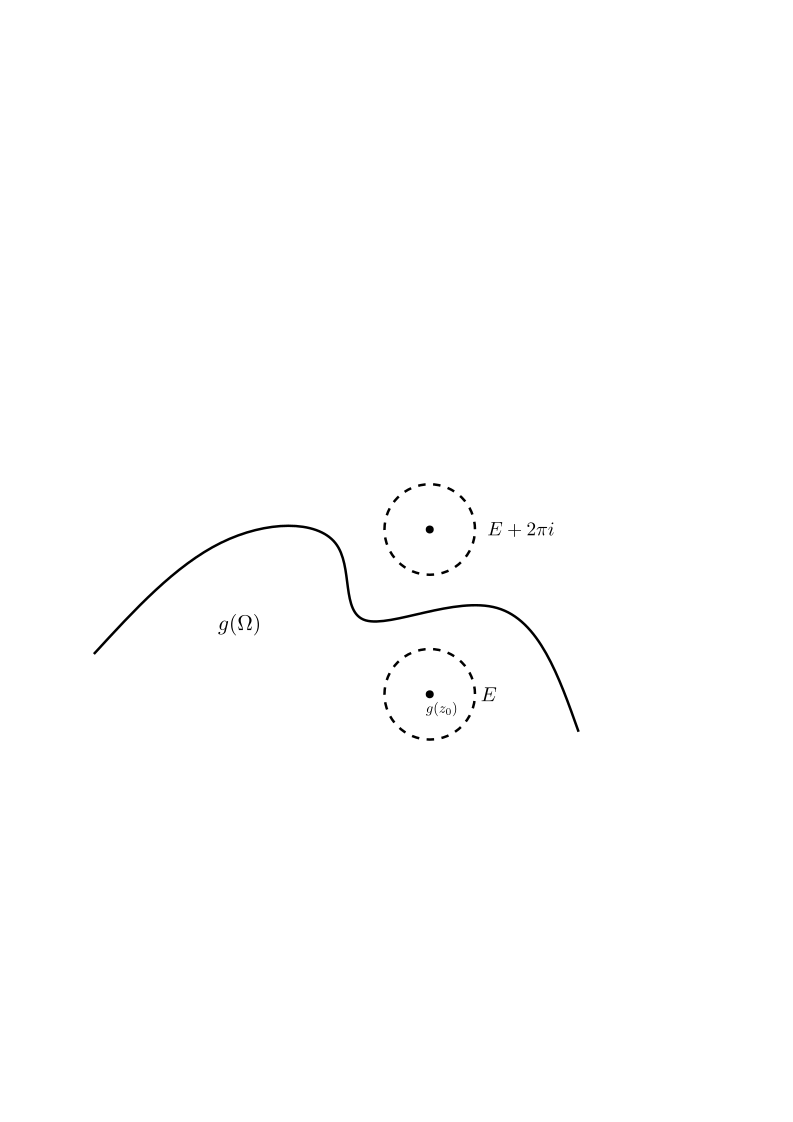
\includegraphics[scale=0.85]{Images/riem_map_pf_2.png}
        \caption{The discs $E$ and $E + 2\pi i$ are disjoint}
        \label{fig:riem-map-pf-2}
    \end{figure}

    We begin by defining a family of functions
    $$\mathscr{A} := \{f \in \Hom(\Omega) : f \text{ is 1-1}, f(0) = 0, f(\Omega) \subset D\}$$
    We will prove the following two lemmas about this family which immediately give us the biholomorphism $g: \Omega \to D$ (the first lemma gives a criterion for when the image of a map in $\mathscr{A}$ is $D$ and the second lemma tells us there is a function satisfying the criterion). 
    \begin{lemma}
        Let $g \in \mathscr{A}$. Then $g(\Omega) = D$ if and only if $\abs{g'(0)} = \sup_{f \in \mathscr{A}} \abs{f'(0)}$.
    \end{lemma}
    \begin{proof}
        Suppose $g(\Omega) = D$. Let $f \in \mathscr{A}$. Take $h = f \circ g^{-1}$ which is a map from the disk to itself which fixes the origin. Then by Schwarz's Lemma we have $\abs{h'(0)} \leq 1$ and hence $\abs{f'(0)} \leq \abs{g'(0)}$. 

        For the converse suppose we have $f \in \mathscr{A}$ such that $f(\Omega) \subsetneq D$. Then we will find a $g \in \mathscr{A}$ such that $\abs{g'(0)} > \abs{f'(0)}$. Then let $a \in D \setminus f(\Omega)$. Define
        $$\varphi(\zeta) = \frac{\zeta - a}{1 - \ol{a} \zeta}$$
        Then
        $$(\varphi \circ f)(z) = \frac{f(z) - a}{1 - \ol{a}f(z)}$$
        is a non-vanishing function on a simply connected region $\Omega$ and hence has a well-defined holomorphic square root, say $F(z)$. This means that $(\varphi \circ f)(z) = F(z)^2$. Define $\theta(z) = z^2$ so that 
        \begin{align*}
            f(z) &= (\varphi^{-1} \circ \theta \circ F)(z)\\ 
            &= \underbrace{(\varphi^{-1} \circ \theta \circ \psi^{-1})}_{h} \circ \underbrace{(\psi \circ F)}_{g}(z)
        \end{align*}
        where
        $$\psi(\eta) = \frac{\eta - F(0)}{1 - \ol{F(0)}\eta}$$
        Then we define $g = \psi \circ F$ and $h = \varphi^{-1} \circ \theta \circ \psi^{-1}$. Notice that $h$ is a holomorphic map from the disk to itself that fixes the origin. Then by Schwarz's lemma we have $\abs{h'(0)} \leq 1$. If we had $\abs{h'(0)} = 1$ then $h$ would be a biholomorphism (in fact by Schwarz we would conclude that it is a rotation of the disk). But we know this cannot be the case since $\theta$ is not a biholomorphism while $\varphi$ and $\psi$ are. Therefore we must have $\abs{h'(0)} < 1$. Writing $h = f \circ g^{-1}$, just as before we conclude via the chain rule that 
        $$\abs{f'(0)} < \abs{g'(0)}$$
    \end{proof}
    
    \begin{lemma}
        There is some $g \in \mathscr{A}$ such that $\abs{g'(0)} = \sup_{f \in \mathscr{A}} \abs{f'(0)}$.
    \end{lemma}
    \begin{proof}
        We know that $\sup \abs{f'(0)}$ must be at least 1 since $\mathscr{A}$ contains the identity. Therefore it suffices to show that 
        $$\mathscr{B} := \{ f \in \mathscr{A} : \abs{f'(0)} \geq 1 \}$$
        is closed in $\Hom(\Omega)$ since that would mean that in particular it contains a function which achieves the supremum. Therefore suppose we have a sequence of functions $f_n \in \mathscr{B}$ that converge to $f$. We want to verify that $f \in \mathscr{B}$. We immediately see that $f(0) = \lim f_n(0) = 0$. Moreover $\abs{f'(0)} = \lim \abs{f_n'(0)} \geq 1$. In particular this means that $f$ is not constant and so by Hurwitz's lemma (see \autoref{cor:hurwitz-cor}) we know that $f$ must also be 1-1. Finally since $\abs{f_n(z)} < 1$ we know that $\abs{f(z)} \leq 1$ for $z \in \Omega$. However if $\abs{f(z)} = 1$ for some $z$ then the Maximum Modulus Principle would imply that $f$ is constant. Therefore $f(\Omega) \subset D$. 
    \end{proof}
    The two lemmas combined show there exists a biholomorphism from $\Omega$ to $D$.
\end{proof}

\subsection{Boundary Behaviour}
We have seen above that if $\Omega$ is a simply connected, proper open subset of $\C$ then there exists a biholomorphism from $\Omega$ to the unit disk $D$. The question then becomes how this biholomorphism behaves on the boundary. We have the following theorem from Carathéodory.
\begin{theorem}[Carathéodory's Theorem]
    A biholomorphism from a simply connected domain $f: \Omega \to D$ extends homeomorphically to the closures $\ol{f}: \ol{\Omega} \to \ol{D}$ if and only if $\partial \Omega$ is a Jordan curve (i.e. homeomorphic to $S^1$).
\end{theorem}

We will not prove the general case but restrict ourselves to the case of a polygon and in fact construct an explicit formula for the inverse. So suppose $\partial \Omega$ is a closed polygonal curve and let $z_1, \dots, z_n$ be the vertices (with $z_{n + 1} = z_1$ due to cyclicity). Suppose we denote the inner angles of the polygons as $\alpha_k \pi$. Therefore we have 
$$\alpha_k \pi = \arg \left( \frac{z_{k - 1} - z_k}{z_{k + 1} - z_k} \right)$$
Let $\beta_k \pi$ be the outer angles so $\beta_k \pi = \pi - \alpha_k \pi = \pi(1 - \alpha_k)$. We know that the sum of the exterior angles of a polygon is always $2\pi$ which means we have $\sum \beta_k = 2$. $\Omega$ is convex if and only if all $\beta_k > 0$.

\begin{figure}[ht]
    \centering
    \includegraphics[scale=0.9]{Images/riem_map_poly_diag.png}
    \caption{The interior angles of our polygon are $\alpha_k \pi$ and the exterior angles are $\beta_k \pi$}
    \label{fig:riem-map-poly-diag}
\end{figure}

First we want to show that any extension should map the boundary to the boundary. In particular, if $\{z_n\}$ is a sequence of points in $\Omega$ that approaches the boundary then $\{f(z_n)\}$ approaches the boundary of $f(\Omega)$ (in fact we don't even need $f$ to be holomorphic for this. Simple continuity is sufficient). First we should make precise what it means to approach the boundary. We say that $\{z_n\} \subset \Omega$ approaches the boundary of $\Omega$ if it is eventually away from every point in $\Omega$, i.e. for every $z \in \Omega$ there exists some $\epsilon > 0$ and $n_0$ such that $\abs{z - z_n} \geq \epsilon$ for all $n \geq n_0$. 

\begin{lemma}
    Suppose $\Omega, \Omega'$ are regions whose boundary is a Jordan curve. Let $f: \Omega \to \Omega'$ be a continuous, surjective map. If $\{z_n\}$ approaches the boundary of $\Omega$ then $\{f(z_n)\}$ approaches the boundary of $\Omega'$. 
\end{lemma}
\begin{proof}
    Let $K$ be a compact subset of $\Omega'$. Then $f^{-1}(K)$ is compact (it's closed by continuity and bounded since $\Omega$ itself is bounded). For every $z \in \Omega$, there exists some $\epsilon$ such that the disk of radius $\epsilon$ centered at $z$ does not contain the tail of $\{z_n\}$. Compactness of $f^{-1}(K)$ implies that it can be covered by finitely many such disks. Then there is a maximum $n_0$ such that $z_n$ for $n \geq n_0$ are all outside the union of these disks. Therefore $f(z_n)$ for $n \geq n_0$ are outside of $K$. We finish the proof by taking $K$ to be a closed disk (that is contained in $\Omega'$) centered at $w \in \Omega'$. 
\end{proof}

Let $f$ be the biholomorphism from the simply connected space $\Omega$ to the unit disk $D$. Let $x_0$ be a non-vertex point on the boundary. By rotating and translating if necessary we can assume that the edge that $x_0$ lies on is on the real axis and the polygon lies in the upper half-plane. Consider a small disk centered at $x_0$ so that $f$ is never 0 on the disk (since $f$ is a biholomorphism onto the unit disk, it is zero at exactly one point so by making the disk small enough we can avoid it). Then $\log f(z)$ has a holomorphic branch on the upper half of this disk. Notice that as $z$ approaches the real axis, $f(z)$ approaches the unit circle by the above lemma. Therefore $\log \abs{f(z)}$ approaches 0. Therefore the real part of the $\log f(z)$ extends continuously to the real axis (in particular it extends to be 0 there). We can then apply the reflection principle to conclude that $\log f(z)$ has a holomorphic extension onto the entire disk and therefore so does $f(z)$. This shows that $f$ extends continuously to the open edges of the polygon and in fact even extends slightly beyond in a holomorphic manner (see \autoref{fig:riem-map-pol-open-edges}). 

A priori, it is possible that because we are only checking for extensions locally on the boundary, we might get conflicting answers if a point lies in two of the above chosen disks. However the extensions will need to agree on $\Omega$ and therefore by the principle of analytic continuation they will agree everywhere on the intersection, in particular on $\partial \Omega$. 

\begin{figure}[ht]
    \centering
    \includegraphics[scale=0.8]{Images/riem_map_poly_open_edges.png}
    \caption{The map $f$ can be extended across edges of the polygon}
    \label{fig:riem-map-pol-open-edges}
\end{figure}

We are then only left with the vertices. We can deal with them in a similar manner but first we will need to `open' them. Suppose we have a small disk $D$ around $z_k$. Then its intersection with $\Omega$ form a small sector. We can map this sector to a half-disk via the map $\zeta = (z - z_k)^{1/\alpha_k}$. Equivalently the map $z = z_k + \zeta^{\alpha_k}$ maps a small half-disk to the sector (for an appropriately chosen branch of $\zeta^{\alpha_k}$). In particular then we have a map from the disk half-disk to the polygon given by $g(\zeta) = f(z_k + \zeta^{\alpha_k})$. By the same argument as before, using the reflection principle we can extend $g$ to a function on the entire disk. Therefore $f$ can be extended around the vertex $z_k$. The same argument holds for all the vertices allowing us to conclude that $f$ extends continuously to the boundary (see \autoref{fig:riem-map-poly-vertex}).

\begin{figure}[ht]
    \centering
    \includegraphics[scale=0.75]{Images/riem_map_poly_vertex.png}
    \caption{We open up the sector at a vertex and then use the same argument as before to extend below the upper half plane}
    \label{fig:riem-map-poly-vertex}
\end{figure}


Finally we want to check that this extension is still 1-1 on the boundary. If we denote the boundary by $\gamma$, we have that
\begin{align*}
    \int_{f \circ \gamma} \frac{1}{z}dz = \int_\gamma \frac{df}{f} = 1
\end{align*}
where the final equality follows from the argument principle (there are no poles in $\Omega$ and exactly one zero since we map biholomorphically onto the unit disk). This means that $f \circ \gamma$ is a closed curved contained in the unit circle with winding number 1. Therefore $f \circ \gamma$ is homotopic to the unit circle. We want to argue that it is exactly the unit circle. For this we consider behaviour of $\arg f(z)$. 

Recall that near any point on the open edge, we have a holomorphic branch of $\log f(z)$. Assuming that this neighbourhood lies in the upper half plane, we know that for as $y$ decreases to 0, we have $\log \abs{f(x + iy)}$ increases to 0.  Then by the Cauchy-Riemann equations, we conclude 
\begin{align*}
    0 > \frac{\partial \log \abs{f}}{\partial y} = -\frac{\partial \arg f}{\partial x}
\end{align*}
In particular then as $z$ travels along an open edge of $\Omega$, $\arg f(z)$ is constantly increasing. Therefore $f \circ \gamma$ is a closed curved homoptopic to unit circle and is such that its argument is constant increasing. It must then be the unit circle exactly. Thus we see that the biholomorphic map from the polygon $\Omega$ to unit disk extends to a homeomorphism of the closures of the respective spaces.
